%\documentclass[ignorenonframetext, compress, 9pt, xcolor=svgnames]{beamer} 
\documentclass[notes, ignorenonframetext, compress, 10pt, xcolor=svgnames, aspectratio=169]{beamer} 
\usepackage{pgfpages}
\usepackage{pdfpages}
% These slides also contain speaker notes. You can print just the slides,
% just the notes, or both, depending on the setting below. Comment out the want
% you want.
\setbeameroption{hide notes} % Only slide
%\setbeameroption{show only notes} % Only notes
%\setbeameroption{show notes on second screen=right} % Both
\usepackage{amsmath}
\usepackage{amsfonts}
\usepackage{amssymb}
\setbeamercolor{frametitle}{fg=MidnightBlue}

\setbeamercolor{sectionpage title}{bg=MidnightBlue}
\setbeamertemplate{frametitle}[default][center]
%\setbeamertemplate{headline}{\vskip2cm}
%\setbeamertemplate{frametitle}{\color{MidnightBlue}\centering\bfseries\insertframetitle\par\vskip-6pt}
\setbeamerfont{frametitle}{series=\bfseries}
\setbeamerfont{title}{series=\bfseries}
\setbeamerfont{sectionpage}{series=\bfseries}
%\setbeamercolor{section in head/foot}{bg=MidnightBlueBlue}
%\setbeamercolor{author in head/foot}{bg=DarkBlue}
\setbeamercolor{author in head/foot}{fg=MidnightBlue}
%\setbeamercolor{title in head/foot}{bg=White}
\setbeamercolor{title in head/foot}{fg=MidnightBlue}
\setbeamercolor{title}{fg=MidnightBlue}
%\setbeamercolor{date in head/foot}{fg=Brown}
%\setbeamercolor{alerted text}{fg=DarkBlue}
%\usecolortheme[named=DarkBlue]{structure} 
%\usepackage{bbm}
%\usepackage{bbold}
\usepackage{eurosym}
\usepackage{graphicx}
%\usepackage{epstopdf}
\usepackage{hyperref}
\hypersetup{
  colorlinks   = true, %Colours links instead of ugly boxes
  urlcolor     = gray, %Colour for external hyperlinks
  linkcolor    = MidnightBlue, %Colour of internal links
  citecolor   = DarkRed %Colour of citations
}
\usepackage{multirow}
\usepackage{xspace}
\usepackage{listings}
\usepackage{natbib}
%\usepackage[sort&compress,comma,super]{natbib}
\def\newblock{} % To avoid a compilation error about a function \newblock undefined
\usepackage{bibentry}
\usepackage{booktabs}
\usepackage{dcolumn}
\usepackage[greek,frenchb]{babel}
\usepackage[babel=true,kerning=true]{microtype}
\usepackage[utf8]{inputenc}
\usepackage[T1]{fontenc}
\usepackage{natbib}
\renewcommand{\cite}{\citet}
\usepackage{longtable}
\usepackage{eso-pic}

\usepackage{xcolor}
 \colorlet{linkequation}{DarkRed} 
 \newcommand*{\SavedEqref}{}
 \let\SavedEqref\eqref 
\renewcommand*{\eqref}[1]{%
\begingroup \hypersetup{
      linkcolor=linkequation,
linkbordercolor=linkequation, }%
\SavedEqref{#1}%
 \endgroup
}

\newcommand*{\refeq}[1]{%
 \begingroup
\hypersetup{ 
linkcolor=linkequation, 
linkbordercolor=linkequation,
}%
\ref{#1}%
 \endgroup
}

\setbeamertemplate{caption}[numbered]
\setbeamertemplate{theorem}[ams style]
\setbeamertemplate{theorems}[numbered]
%\usefonttheme{serif}
%\usecolortheme{beaver}
%\usetheme{Hannover}
%\usetheme{CambridgeUS}
%\usetheme{Madrid}
%\usecolortheme{whale}
%\usetheme{Warsaw}
%\usetheme{Luebeck}
%\usetheme{Montpellier}
%\usetheme{Berlin}
%\setbeamercolor{titlelike}{parent=structure}
%\setbeamertemplate{headline}[default]
%\setbeamertemplate{footline}[default]
%\setbeamertemplate{footline}[Malmoe]
%\setbeamercovered{transparent}
%\setbeamercovered{invisible}
%\usecolortheme{crane}
%\usecolortheme{dolphin}
%\usepackage{pxfonts}
%\usepackage{isomath}
%\usepackage{mathpazo}
%\usepackage{arev} %     (Arev/Vera Sans)
%\usepackage{eulervm} %_   (Euler Math)
%\usepackage{fixmath} %  (Computer Modern)
%\usepackage{hvmath} %_   (HV-Math/Helvetica)
%\usepackage{tmmath} %_   (TM-Math/Times)
%\usepackage{tgheros}
%\usepackage{cmbright}
%\usepackage{ccfonts} \usepackage[T1]{fontenc}
%\usepackage[garamond]{mathdesign}

%\usepackage{color}
%\usepackage{ulem}

%\usepackage[math]{kurier}
%\usepackage[no-math]{fontspec}
%\setmainfont{Fontin Sans}
%\setsansfont{Fontin Sans}
%\setbeamerfont{frametitle}{size=\LARGE,series=\bfseries}
%%%add 19022021
\usepackage{enumerate}    
\usepackage{dcolumn}
\usepackage{verbatim}
\newcolumntype{d}[0]{D{.}{.}{5}}
%\setbeamertemplate{note page}{\pagecolor{yellow!5}\insertnote}
%\usetikzlibrary{positioning}
%\usetikzlibrary{snakes}
%\usetikzlibrary{calc}
%\usetikzlibrary{arrows}
%\usetikzlibrary{decorations.markings}
%\usetikzlibrary{shapes.misc}
%\usetikzlibrary{matrix,shapes,arrows,fit,tikzmark}
%%%
% suppress navigation bar
\beamertemplatenavigationsymbolsempty
%\usetheme{bunsenMod}
%\setbeamercovered{transparent}
%\setbeamertemplate{items}[circle]
%\usecolortheme[named=CadetBlue]{structure}
%\usecolortheme[RGB={225,64,5}]{structure}
%\definecolor{burntRed}{RGB}{225,64,5}
%\setbeamercolor{alerted text}{fg=burntRed} 
%\usecolortheme[RGB={0,40,110}]{structure}
%\hypersetup{linkcolor=burntRed}
%\hypersetup{urlcolor=burntRed}
%\hypersetup{filecolor=burntRed}
%\hypersetup{citecolor=burntRed}

%\usetheme{bunsenMod}
%\setbeamercovered{transparent}
%\setbeamertemplate{items}[circle]
%\usecolortheme[named=CadetBlue]{structure}
%\usecolortheme[RGB={225,64,5}]{structure}
%\definecolor{burntRed}{RGB}{225,64,5}
%\setbeamercolor{alerted text}{fg=burntRed} 
%\usecolortheme[RGB={0,40,110}]{structure}
%\hypersetup{linkcolor=burntRed}
%\hypersetup{urlcolor=burntRed}
%\hypersetup{filecolor=burntRed}
%\hypersetup{citecolor=burntRed}

%\AtBeginSection[] % Do nothing for \section*
%{ \frame{\sectionpage} }
%\setbeamertemplate{frametitle continuation}{}
\newtheorem{lemme}{Lemme}[section]
%\newtheorem{remarque}{Remarque}
\newcommand{\argmax}{\operatornamewithlimits{arg\,max}}
\newcommand{\argmin}{\operatornamewithlimits{arg\,min}}
\def\inprobLOW{\rightarrow_p}
\def\inprobHIGH{\,{\buildrel p \over \rightarrow}\,} 
\def\inprob{\,{\inprobHIGH}\,} 
\def\indist{\,{\buildrel d \over \rightarrow}\,} 
\def\sima{\,{\buildrel a \over \sim}\,} 
\def\F{\mathbb{F}}
\def\R{\mathbb{R}}
\def\N{\mathbb{N}}
\newcommand{\gmatrix}[1]{\begin{pmatrix} {#1}_{11} & \cdots &
    {#1}_{1n} \\ \vdots & \ddots & \vdots \\ {#1}_{m1} & \cdots &
    {#1}_{mn} \end{pmatrix}}
\newcommand{\iprod}[2]{\left\langle {#1} , {#2} \right\rangle}
\newcommand{\norm}[1]{\left\Vert {#1} \right\Vert}
\newcommand{\abs}[1]{\left\vert {#1} \right\vert}
\renewcommand{\det}{\mathrm{det}}
\newcommand{\rank}{\mathrm{rank}}
\newcommand{\spn}{\mathrm{span}}
\newcommand{\row}{\mathrm{Row}}
\newcommand{\col}{\mathrm{Col}}
\renewcommand{\dim}{\mathrm{dim}}
\newcommand{\prefeq}{\succeq}
\newcommand{\pref}{\succ}
\newcommand{\seq}[1]{\{{#1}_n \}_{n=1}^\infty }
\renewcommand{\to}{{\rightarrow}}
\renewcommand{\L}{{\mathcal{L}}}
\newcommand{\Er}{\mathrm{E}}
\renewcommand{\Pr}{\mathrm{P}}
%\newcommand{\Var}{\mathrm{Var}}
%\newcommand{\Cov}{\mathrm{Cov}}
%\newcommand{\corr}{\mathrm{Corr}}
%\newcommand{\Var}{\mathrm{Var}}
\newcommand{\bias}{\mathrm{Bias}}
\newcommand{\mse}{\mathrm{MSE}}
\providecommand{\Pred}{\mathcal{P}}
\providecommand{\plim}{\operatornamewithlimits{plim}}
\providecommand{\avg}{\frac{1}{n} \underset{i=1}{\overset{n}{\sum}}}
\providecommand{\sumin}{{\sum_{i=1}^n}}
\providecommand{\sumiN}{{\sum_{i=1}^N}}
\providecommand{\sumtT}{{\sum_{t=1}^T}}
\providecommand{\limp}{\overset{p}{\rightarrow}}
\providecommand{\liml}{\overset{L}{\rightarrow}}
%\providecommand{\limp}{\underset{n \rightarrow \infty}{\overset{p}{\longrightarrow}}}
%\providecommand{\limp}{\underset{n \rightarrow \infty}{\overset{p}{\longrightarrow}}}
%\providecommand{\limp}{\overset{p}{\longrightarrow}}
%\providecommand{\limd}{\underset{n \rightarrow \infty}{\overset{d}{\longrightarrow}}}
\providecommand{\limd}{\overset{d}{\rightarrow}}
\providecommand{\limps}{\overset{p.s.}{\rightarrow}}
\providecommand{\limlp}{\overset{L^p}{\rightarrow}}
\providecommand{\limprob}{\overset{p}{\underset{N\to +\infty}{\longrightarrow}}}
\providecommand{\limloi}{\overset{L}{\underset{N\to +\infty}{\longrightarrow}}}
\providecommand{\limpsure}{\overset{p.s.}{\underset{N\to +\infty}{\longrightarrow}}}
\def\independenT#1#2{\mathrel{\setbox0\hbox{$#1#2$}%
    \copy0\kern-\wd0\mkern4mu\box0}} 
\newcommand\indep{\protect\mathpalette{\protect\independenT}{\perp}}


\lstset{language=R}
\lstset{keywordstyle=\color[rgb]{0,0,1},                                        % keywords
        commentstyle=\color[rgb]{0.133,0.545,0.133},    % comments
        stringstyle=\color[rgb]{0.627,0.126,0.941}      % strings
}       
\lstset{
  showstringspaces=false,       % not emphasize spaces in strings 
  columns=fixed,
  numbersep=3mm, numbers=left, numberstyle=\tiny,       % number style
  frame=none,
  framexleftmargin=5mm, xleftmargin=5mm         % tweak margins
}
\makeatletter
%\setbeamertemplate{frametitle continuation}{\gdef\beamer@frametitle{}}
\setbeamertemplate{frametitle continuation}{\frametitle{}}
%\setbeamertemplate{frametitle continuation}{\insertcontinuationcount}
\makeatother

\theoremstyle{remark}
\newtheorem{interpretation}{Interprétation}
\newtheorem*{interpretation*}{Interprétation}

\theoremstyle{remark}
\newtheorem{remarque}{Remarque}%[section]
\newtheorem*{remarque*}{Remarque}
\usepackage[framemethod=TikZ]{mdframed} 
\usepackage{showexpl}
%\newtheorem{step}{Step}[section]
%\newtheorem{rem}{Comment}[section]
%\newtheorem{ex}{Example}[section]
%\newtheorem{hist}{History}[section]
%\newtheorem*{ex*}{Example}
%\theoremstyle{plain}
%\newtheorem{propriete}{Propri\'et\'e}
%\renewcommand{\thepropriete}{P\arabic{propriete}}
%\theoremstyle{definition}
%\newtheorem{definition}{Définition}%[section]
%\theoremstyle{remark}
%\newtheorem{exemple}{Exemple}
%\newtheorem*{exemple*}{Exemple}

\newtheorem{theoreme}{Théorème}
\newtheorem{proposition}{Proposition}
%\newtheorem{propriete}{Propri\'et\'e}
\newtheorem{corollaire}{Corollaire}
%\newtheorem{exemple}{Exemple}
%\newtheorem{assumption}{Assumption}
%\renewcommand{\theassumption}{A\arabic{assumption}}
\newtheorem{hypothese}{Hypothèse}
\renewcommand{\thehypothese}{H\arabic{hypothese}}
%\theoremstyle{definition}

%\newtheorem{definitionx}{D\'efinition}%[section]
%\newenvironment{definition}
 %{\pushQED{\qed}\renewcommand{\qedsymbol}{$\triangle$}\definitionx}
 %{\popQED\enddefinitionx}

%\newtheorem{condition}{Condition}
%\renewcommand{\thecondition}{C\arabic{condition}}
%\newcommand{\Var}{\mathbb{V}}
%\newcommand{\Var}{\mathbf{Var}}
%\newcommand{\Exp}{\mathbf{E}}
%\providecommand{\Vr}{\mathrm{Var}}
%\renewcommand{\Er}{\mathbb{E}}
%\newcommand{\LP}{\mathcal{LP}}
%\providecommand{\Id}{\mathbf{I}}
%\providecommand{\Rang}{\mathrm{Rang}}
%\providecommand{\Trace}{\mathrm{Trace}}
%\newcommand{\Cov}{\mathbf{Cov}}
%\newcommand{\Cov}{\mathbb{C}\mathrm{ov}}
\providecommand{\Id}{\mathbf{I}}
\providecommand{\Ind}{\mathbf{1}}
\providecommand{\uvec}{\mathbf{1}}
\providecommand{\vecOnes}{\mathbf{1}}
\DeclareMathOperator{\indfun}{\mathbf{1}}
\DeclareMathOperator{\Exp}{E}
\DeclareMathOperator{\Expn}{\mathbb{E}_n}
\DeclareMathOperator{\EL}{EL}
\DeclareMathOperator{\Var}{Var}
\DeclareMathOperator{\Vr}{V}
\newcommand{\boldVr}{ {\boldsymbol \Vr} }
\DeclareMathOperator{\Cov}{Cov}
\DeclareMathOperator{\corr}{corr}
\DeclareMathOperator{\perps}{\perp_s}
%\DeclareMathOperator{\Prob}{Pr}
\DeclareMathOperator{\Prob}{P}
\DeclareMathOperator{\prob}{p}
\DeclareMathOperator{\loss}{L}
\providecommand{\Corr}{\mathrm{Corr}}
\providecommand{\Diag}{\mathrm{Diag}}
\providecommand{\reg}{\mathrm{r}}
\providecommand{\Likelihood}{\mathrm{L}}
\renewcommand{\Pr}{{\mathbb{P}}}
\providecommand{\set}[1]{\left\{#1\right\}}
\providecommand{\uvec}{\mathbf{1}}
\providecommand{\Rang}{\mathrm{Rang}}
\providecommand{\Trace}{\mathrm{Trace}}
\providecommand{\Tr}{\mathrm{Tr}}
\providecommand{\CI}{\mathrm{CI}}
\providecommand{\asyvar}{\mathrm{AsyVar}}
\DeclareMathOperator{\Supp}{Supp}
\newcommand{\inputslide}[2]{{
    \usebackgroundtemplate{
     \includegraphics[page={#2},width=0.90\textwidth,keepaspectratio=true]
      %\includegraphics[page={#2},width=\paperwidth,keepaspectratio=true]
      {{#1}}}
    \frame[plain]{}
  }}
\newcommand\pperp{\perp\!\!\!\perp}
\newcommand\independent{\protect\mathpalette{\protect\independenT}{\perp}}
\def\independenT#1#2{\mathrel{\rlap{$#1#2$}\mkern2mu{#1#2}}}
\usepackage{bbm}
\providecommand{\Ind}{\mathbf{1}}
\newcommand{\sumjsi}{\underset{i<j}{{\sum}}}
\newcommand{\prodjsi}{\underset{i<j}{{\prod}}}
\newcommand{\sumisj}{\underset{j<i}{{\sum}}}
\newcommand{\prodisj}{\underset{j<i}{{\prod}}}
\newcommand{\sumobs}{\underset{i=1}{\overset{n}{\sum}}}
\newcommand{\sumi}{\underset{i=1}{\overset{n}{\sum}}}
\newcommand{\prodi}{\underset{i=1}{\overset{n}{\prod}}}
\newcommand{\prodobs}{\underset{i=1}{\overset{n}{\prod}}}
\newcommand{\simiid}{{\overset{i.i.d.}{\sim}}}
%\newcommand{\sumobs}{\sum_{i=1}^N}
%\newcommand{\prodobs}{\prod_{i=1}^N}
%\newcommand{\sumjsi}{\sum_{i<j}}
%\newcommand{\prodjsi}{\prod_{i<j}}
%\newcommand{\sumisj}{\sum_{j<i}}
%\newcommand{\prodisj}{\sum_{j<i}}

%\usepackage{appendixnumberbeamer}
\setbeamertemplate{footline}[frame number]
\setbeamertemplate{section in toc}[sections numbered]
\setbeamertemplate{subsection in toc}[subsections numbered]
\setbeamertemplate{subsubsection in toc}[subsubsections numbered]

%\makeatother
%\setbeamertemplate{footline}
%{
%    \leavevmode%
%    \hbox{%
%        \begin{beamercolorbox}[wd=.333333\paperwidth,ht=2.25ex,dp=1ex,center]{author in head/foot}%
%            \usebeamerfont{author in head/foot}\insertshortauthor
%        \end{beamercolorbox}%
%        \begin{beamercolorbox}[wd=.333333\paperwidth,ht=2.25ex,dp=1ex,center]{title in head/foot}%
%            \usebeamerfont{title in head/foot}\insertshorttitle
%        \end{beamercolorbox}%
%        \begin{beamercolorbox}[wd=.333333\paperwidth,ht=2.25ex,dp=1ex,right]{date in head/foot}%
%            \usebeamerfont{date in head/foot}\insertshortdate{}\hspace*{2em}
%            \insertframenumber{} / \inserttotalframenumber\hspace*{2ex} 
%        \end{beamercolorbox}}%
%       \vskip0pt%
 %   }
%   \makeatother
%\setbeamertemplate{navigation symbols}{}
\setbeamertemplate{itemize items}[ball]
%\setbeamertemplate{itemize items}{-}
%\newenvironment{wideitemize}{\itemize\addtolength{\itemsep}{10pt}}{\enditemize}
% \usepackage{eso-pic}
%\newcommand\AtPagemyUpperLeft[1]{\AtPageLowerLeft{%
%\put(\LenToUnit{0.9\paperwidth},\LenToUnit{0.9\paperheight}){#1}}}
%\AddToShipoutPictureFG{
%  \AtPagemyUpperLeft{{\includegraphics[width=1.1cm,keepaspectratio]{../logo-uga.png}}}
%}%
\def\figheight{3in}
\def\figwidth{4in}

%%Commands from Econometric Theory(Slides) by J. Stachurski.

\newcommand{\boldx}{ {\mathbf x} }
\newcommand{\boldu}{ {\mathbf u} }
\newcommand{\boldv}{ {\mathbf v} }
\newcommand{\boldw}{ {\mathbf w} }
\newcommand{\boldy}{ {\mathbf y} }
\newcommand{\boldb}{ {\mathbf b} }
\newcommand{\bolda}{ {\mathbf a} }
\newcommand{\boldc}{ {\mathbf c} }
\newcommand{\boldd}{ {\mathbf d} }
\newcommand{\boldi}{ {\mathbf i} }
\newcommand{\bolde}{ {\mathbf e} }
\newcommand{\boldp}{ {\mathbf p} }
\newcommand{\boldq}{ {\mathbf q} }
\newcommand{\bolds}{ {\mathbf s} }
\newcommand{\boldt}{ {\mathbf t} }
\newcommand{\boldz}{ {\mathbf z} }
\newcommand{\boldr}{ {\mathbf r} }
\newcommand{\boldm}{ {\mathbf m} }

\newcommand{\boldzero}{ {\mathbf 0} }
\newcommand{\boldone}{ {\mathbf 1} }

\newcommand{\boldalpha}{ {\boldsymbol \alpha} }
\newcommand{\boldbeta}{ {\boldsymbol \beta} }
\newcommand{\boldgamma}{ {\boldsymbol \gamma} }
\newcommand{\boldGamma}{ {\boldsymbol \Gamma} }
\newcommand{\boldtheta}{ {\boldsymbol \theta} }
\newcommand{\boldxi}{ {\boldsymbol \xi} }
\newcommand{\boldtau}{ {\boldsymbol \tau} }
\newcommand{\boldepsilon}{ {\boldsymbol \epsilon} }
\newcommand{\boldvepsilon}{ {\boldsymbol \varepsilon} }
\newcommand{\boldmu}{ {\boldsymbol \mu} }
\newcommand{\boldSigma}{ {\boldsymbol \Sigma} }
\newcommand{\boldOmega}{ {\boldsymbol \Omega} }
\newcommand{\boldPhi}{ {\boldsymbol \Phi} }
\newcommand{\boldLambda}{ {\boldsymbol \Lambda} }
\newcommand{\boldphi}{ {\boldsymbol \phi} }
\newcommand{\boldeta}{ {\boldsymbol \eta} }

\newcommand{\Sigmax}{ {\boldsymbol \Sigma_{\boldx}}}
\newcommand{\Sigmau}{ {\boldsymbol \Sigma_{\boldu}}}
\newcommand{\Sigmaxinv}{ {\boldsymbol \Sigma_{\boldx}^{-1}}}
\newcommand{\Sigmav}{ {\boldsymbol \Sigma_{\boldv \boldv}}}

\newcommand{\hboldx}{ \hat {\mathbf x} }
\newcommand{\hboldy}{ \hat {\mathbf y} }
\newcommand{\hboldb}{ \hat {\mathbf b} }
\newcommand{\hboldu}{ \hat {\mathbf u} }
\newcommand{\hboldtheta}{ \hat {\boldsymbol \theta} }
\newcommand{\hboldtau}{ \hat {\boldsymbol \tau} }
\newcommand{\hboldmu}{ \hat {\boldsymbol \mu} }
\newcommand{\hboldbeta}{ \hat {\boldsymbol \beta} }
\newcommand{\hboldgamma}{ \hat {\boldsymbol \gamma} }
\newcommand{\hboldSigma}{ \hat {\boldsymbol \Sigma} }

\newcommand{\boldA}{\mathbf A}
\newcommand{\boldB}{\mathbf B}
\newcommand{\boldC}{\mathbf C}
\newcommand{\boldD}{\mathbf D}
\newcommand{\boldI}{\mathbf I}
\newcommand{\boldL}{\mathbf L}
\newcommand{\boldM}{\mathbf M}
\newcommand{\boldP}{\mathbf P}
\newcommand{\boldQ}{\mathbf Q}
\newcommand{\boldR}{\mathbf R}
\newcommand{\boldX}{\mathbf X}
\newcommand{\boldU}{\mathbf U}
\newcommand{\boldV}{\mathbf V}
\newcommand{\boldW}{\mathbf W}
\newcommand{\boldY}{\mathbf Y}
\newcommand{\boldZ}{\mathbf Z}

\newcommand{\bSigmaX}{ {\boldsymbol \Sigma_{\hboldbeta}} }
\newcommand{\hbSigmaX}{ \mathbf{\hat \Sigma_{\hboldbeta}} }
\newcommand{\betahat}{\hat{\beta}}
\newcommand{\gammahat}{\hat{\gamma}}
\newcommand{\Uhat}{\hat{U}}
\newcommand{\Vhat}{\hat{V}}
\newcommand{\epsilonhat}{\hat{\epsilon}}
\newcommand{\sigmahat}{\hat{\sigma}}
\newcommand{\Sigmahat}{\hat{\Sigma}}
\newcommand{\Gammahat}{\hat{\Gamma}}

\newcommand{\RR}{\mathbbm R}
\newcommand{\CC}{\mathbbm C}
\newcommand{\NN}{\mathbbm N}
\newcommand{\PP}{\mathbbm P}
\newcommand{\EE}{\mathbbm E \nobreak\hspace{.1em}}
\newcommand{\EEP}{\mathbbm E_P \nobreak\hspace{.1em}}
\newcommand{\ZZ}{\mathbbm Z}
\newcommand{\QQ}{\mathbbm Q}


\newcommand{\XX}{\mathbbm X}

\newcommand{\aA}{\mathcal A}
\newcommand{\fF}{\mathscr F}
\newcommand{\bB}{\mathscr B}
\newcommand{\iI}{\mathscr I}
\newcommand{\rR}{\mathscr R}
\newcommand{\dD}{\mathcal D}
\newcommand{\lL}{\mathcal L}
\newcommand{\llL}{\mathcal{H}_{\ell}}
\newcommand{\gG}{\mathcal G}
\newcommand{\hH}{\mathcal H}
\newcommand{\nN}{\textrm{\sc n}}
\newcommand{\lN}{\textrm{\sc ln}}
\newcommand{\pP}{\mathscr P}
\newcommand{\qQ}{\mathscr Q}
\newcommand{\xX}{\mathcal X}
\newcommand{\yY}{\mathcal Y}
\newcommand{\ddD}{\mathscr D}


%\newcommand{\R}{{\texttt R}}
\newcommand{\risk}{\mathcal R}
\newcommand{\Remp}{R_{{\rm emp}}}

\newcommand*\diff{\mathop{}\!\mathrm{d}}
\newcommand{\ess}{ \textrm{{\sc ess}} }
\newcommand{\tss}{ \textrm{{\sc tss}} }
\newcommand{\rss}{ \textrm{{\sc rss}} }
\newcommand{\rssr}{ \textrm{{\sc rssr}} }
\newcommand{\ussr}{ \textrm{{\sc ussr}} }
\newcommand{\zdata}{\mathbf{z}_{\mathcal D}}
\newcommand{\Pdata}{P_{\mathcal D}}
\newcommand{\Pdatatheta}{P^{\mathcal D}_{\theta}}
\newcommand{\Zdata}{Z_{\mathcal D}}


\newcommand{\e}[1]{\mathbbm{E}[{#1}]}
\newcommand{\p}[1]{\mathbbm{P}({#1})}

% condition
\theoremstyle{definition}
\newtheorem{condition}{Condition}
\renewcommand{\thecondition}{C\arabic{condition}}
\BeforeBeginEnvironment{condition}{
  \setbeamerfont{block title}{series=\bfseries}
  \setbeamercolor{block title}{fg=MidnightBlue,bg=white}
  \setbeamercolor{block body}{fg=black, bg=gray!10}
}
\newtheorem*{condition*}{Condition}
\BeforeBeginEnvironment{condition*}{
  \setbeamerfont{block title}{series=\bfseries}
  \setbeamercolor{block title}{fg=MidnightBlue,bg=white}
  \setbeamercolor{block body}{fg=black, bg=gray!10}
}

% assumption
\theoremstyle{definition}
\newtheorem{assumption}{Assumption}
\BeforeBeginEnvironment{assumption}{
  \setbeamerfont{block title}{series=\bfseries}
  \setbeamercolor{block title}{fg=MidnightBlue,bg=white}
  \setbeamercolor{block body}{fg=black, bg=gray!10}
}
\newtheorem*{assumption*}{Assumption}
\BeforeBeginEnvironment{assumption*}{
  \setbeamerfont{block title}{series=\bfseries}
  \setbeamercolor{block title}{fg=MidnightBlue,bg=white}
  \setbeamercolor{block body}{fg=black, bg=gray!10}
}

% definition
\BeforeBeginEnvironment{definition}{
  \setbeamerfont{block title}{series=\bfseries}
  \setbeamercolor{block title}{fg=MidnightBlue,bg=white}
  \setbeamercolor{block body}{fg=black, bg=gray!10}
}
\newtheorem*{definition*}{Definition}
\BeforeBeginEnvironment{definition*}{
  \setbeamerfont{block title}{series=\bfseries}
  \setbeamercolor{block title}{fg=MidnightBlue,bg=white}
  \setbeamercolor{block body}{fg=black, bg=gray!10}
}

% theorem
\theoremstyle{plain}
\BeforeBeginEnvironment{theorem}{
  \setbeamerfont{block body}{shape=\itshape}
  \setbeamerfont{block title}{series=\bfseries}
  \setbeamercolor{block title}{fg=MidnightBlue,bg=white}
  \setbeamercolor{block body}{fg=black, bg=gray!10}
}
\newtheorem*{theorem*}{Theorem}
\BeforeBeginEnvironment{theorem*}{
  \setbeamerfont{block body }{shape=\itshape}
  \setbeamerfont{block title}{series=\bfseries}
  \setbeamercolor{block title}{fg=MidnightBlue,bg=white}
  \setbeamercolor{block body}{fg=black, bg=gray!10}
}

% definition_fr
\theoremstyle{definition}
\newtheorem{definition_fr}{Définition}%[section]
\BeforeBeginEnvironment{definition_fr}{
  \setbeamerfont{block title}{series=\bfseries}
  \setbeamercolor{block title}{fg=MidnightBlue,bg=white}
  \setbeamercolor{block body}{fg=black, bg=gray!10}
}
\newtheorem*{definition_fr*}{Définition}
\BeforeBeginEnvironment{definition_fr*}{
  \setbeamerfont{block title}{series=\bfseries}
  \setbeamercolor{block title}{fg=MidnightBlue,bg=white}
  \setbeamercolor{block body}{fg=black, bg=gray!10}
}
% theorem_fr
\newtheorem{theorem_fr}{Théorème}%[section]
\BeforeBeginEnvironment{theorem_fr}{
  \setbeamerfont{block body}{shape=\itshape}
  \setbeamerfont{block title}{series=\bfseries, shape = \upshape}
  \setbeamercolor{block title}{fg=MidnightBlue,bg=white}
  \setbeamercolor{block body}{fg=black, bg=gray!10}
}
\newtheorem*{theorem_fr*}{Théorème}
\BeforeBeginEnvironment{theorem_fr*}{
  \setbeamerfont{block body}{shape=\itshape}
  \setbeamerfont{block title}{series=\bfseries, shape = \upshape}
  \setbeamercolor{block title}{fg=MidnightBlue,bg=white}
  \setbeamercolor{block body}{fg=black, bg=gray!10}
}

% remark_fr
\theoremstyle{remark}
\newtheorem{remark_fr}{Remarque}%[section]
\BeforeBeginEnvironment{remark_fr}{
  \setbeamerfont{block title}{series=\bfseries, shape=\itshape}
  \setbeamercolor{block title}{fg=MidnightBlue,bg=white}
  \setbeamercolor{block body}{fg=black, bg=gray!10}
}
\newtheorem*{remark_fr*}{Remarque}
\BeforeBeginEnvironment{remark_fr*}{
  \setbeamerfont{block title}{series=\bfseries, shape=\itshape}
  \setbeamercolor{block title}{fg=MidnightBlue,bg=white}
  \setbeamercolor{block body}{fg=black, bg=gray!10}
}

% exemple
\theoremstyle{remark}
\newtheorem{exemple}{Exemple}%[section]
\BeforeBeginEnvironment{exemple}{
  \setbeamerfont{block title}{series=\bfseries, shape=\itshape}
  \setbeamercolor{block title}{fg=MidnightBlue,bg=white}
  \setbeamercolor{block body}{fg=black, bg=gray!10}
}
\newtheorem*{exemple*}{}
\BeforeBeginEnvironment{exemple*}{
  \setbeamerfont{block title}{series=\bfseries, shape=\itshape}
  \setbeamercolor{block title}{fg=MidnightBlue,bg=white}
  \setbeamercolor{block body}{fg=black, bg=gray!10}
}


% propriete
\theoremstyle{plain}
\newtheorem{propriete}{Propri\'et\'e}%[section]
\BeforeBeginEnvironment{propriete}{
  \setbeamerfont{block body}{shape=\itshape}
  \setbeamerfont{block title}{series=\bfseries, shape = \upshape}
  \setbeamercolor{block title}{fg=MidnightBlue,bg=white}
  \setbeamercolor{block body}{fg=black, bg=gray!10}
}
\newtheorem*{propriete*}{Propri\'et\'e}
\BeforeBeginEnvironment{propriete*}{
  \setbeamerfont{block body}{shape=\itshape}
  \setbeamerfont{block title}{series=\bfseries, shape = \upshape}
  \setbeamercolor{block title}{fg=MidnightBlue,bg=white}
  \setbeamercolor{block body}{fg=black, bg=gray!10}
}


% remark
\theoremstyle{remark}
\newtheorem{remark}{Remark}%[section]
\BeforeBeginEnvironment{remark}{
  \setbeamerfont{block body}{shape=\itshape}
  \setbeamerfont{block title}{series=\bfseries}
  \setbeamercolor{block title}{fg=MidnightBlue,bg=white}
  \setbeamercolor{block body}{fg=black, bg=gray!10}
}
\newtheorem*{remark*}{Remark}
\BeforeBeginEnvironment{remark*}{
  \setbeamerfont{block body }{shape=\itshape}
  \setbeamerfont{block title}{series=\bfseries}
  \setbeamercolor{block title}{fg=MidnightBlue,bg=white}
  \setbeamercolor{block body}{fg=black, bg=gray!10}
}


\usepackage[svgnames]{xcolor}
\usepackage{tikz}
\usetikzlibrary{shapes.geometric, arrows}
\usepackage{enumerate}   
\usepackage{multirow}
\usepackage{txfonts}
\usepackage{mathrsfs}
\usepackage{pgfplots}
\pgfplotsset{compat = newest}
\usetikzlibrary{positioning, arrows.meta}
\usepgfplotslibrary{fillbetween}
\newcommand{\A}{(0,0) ++(135:2) circle (2)}
\newcommand{\B}{(0,0) ++(45:2) circle (2)}
\DeclareMathOperator{\C}{C}
\DeclareMathOperator{\util}{u}
%\setbeamersize{text margin left=1.5em,text margin right=1.5em} 
%\setbeamersize{text margin left=1.2cm,text margin right=1.2cm} 
\setbeamersize{text margin left=1.5em,text margin right=1.5em} 
%\usepackage{xr}
%\externaldocument{Econometrie1_UGA_P2e}
  \usepackage{eso-pic}
%\newcommand\AtPagemyUpperLeft[1]{\AtPageLowerLeft{%
%\put(\LenToUnit{0.9\paperwidth},\LenToUnit{0.85\paperheight}){#1}}}
%\AddToShipoutPictureFG{
 % \AtPagemyUpperLeft{{\includegraphics[width=1.1cm,keepaspectratio]{logoUGA2020.pdf}}}
%}%

%\setbeamercolor{title}{fg=black}
%\setbeamercolor{frametitle}{fg=black}
%\setbeamercolor{section in head/foot}{fg=black}
%\setbeamercolor{author in head/foot}{bg=Brown}
%\setbeamercolor{date in head/foot}{fg=Brown}
\AtBeginSection[]
  {
    \ifnum \value{framenumber}>1
      \begin{frame}<beamer>
      \frametitle{PLAN}
      \tableofcontents[currentsection]
      \end{frame}
    \else
    \fi
  }
\setbeamertemplate{section page}
{
    \begin{centering}
    \begin{beamercolorbox}[sep=11pt,center]{part title}
    \usebeamerfont{section title}\thesection.~\insertsection\par
    \end{beamercolorbox}
    \end{centering}
}
%\titlegraphic{\includegraphics[width=1cm]{logoUGA2020.pdf}}
\title[]{ \textbf{ÉCONOMIE INDUSTRIELLE}\footnote{Responsable du cours: Alexis Garapin.}\\(\textbf{UGA, L3 E2AD, S2})}
\subtitle{TRAVAUX DIRIGÉS: TD 1}
\date{\today}
\author{Michal W. Urdanivia\inst{*}}
\institute{\inst{*}UGA, Facult\'e d'\'Economie, GAEL, \\
e-mail:
 \href{
     mailto:michal.wong-urdanivia@univ-grenoble-alpes.fr}{michal.wong-urdanivia@univ-grenoble-alpes.fr}}

%\titlegraphic{\includegraphics[width=1cm]{logoUGA2020.pdf}
%}

\begin{document}

%%% TIKZ STUFF
\usetikzlibrary{positioning}
\usetikzlibrary{snakes}
\usetikzlibrary{calc}
\usetikzlibrary{arrows}
\usetikzlibrary{decorations.markings}
\usetikzlibrary{shapes.misc}
\usetikzlibrary{matrix,shapes,arrows,fit,tikzmark}
\usetikzlibrary{matrix,chains,positioning,decorations.pathreplacing,arrows}
\usetikzlibrary{shapes}
\usetikzlibrary{shapes.geometric, arrows}
\tikzset{   
        every picture/.style={remember picture,baseline},
        every node/.style={anchor=base,align=center,outer sep=1.5pt},
        every path/.style={thick},
        }
\newcommand\marktopleft[1]{
    \tikz[overlay,remember picture] 
        \node (marker-#1-a) at (-.3em,.3em) {};%
}
\newcommand\markbottomright[2]{%
    \tikz[overlay,remember picture] 
        \node (marker-#1-b) at (0em,0em) {};%
}
\tikzstyle{every picture}+=[remember picture] 
\tikzstyle{mybox} =[draw=black, very thick, rectangle, inner sep=10pt, inner ysep=20pt]
\tikzstyle{fancytitle} =[draw=black,fill=red, text=white]
\tikzstyle{observed}=[draw,circle,fill=gray!50]

\begin{frame}
\titlepage
\end{frame}
\begin{frame}
 \tableofcontents
    \end{frame}
%\begin{frame}
%\frametitle{Contenu}
%\tableofcontents[pausesections, pausesubsections]
%\end{frame}

%\section{Qu'est-ce que l’économétrie ? A quoi (à qui) ça sert ?}
%\frame{\sectionpage}
%\begin{frame}
%  \tableofcontents  
%\end{frame}
\section{Introduction}
\frame{\sectionpage}

\begin{frame}
  [allowframebreaks]{Références}
  \begin{itemize}
\item En premier lieu : \href{https://cours.univ-grenoble-alpes.fr/course/view.php?id=5945\#section-2}{Le cours magistral d'Alexis}.
\item Un classique: \cite{Tirole_BookIO_1988}.
\end{itemize}

\end{frame}

\begin{frame}
  [allowframebreaks]{Données de l'exercice}
  \begin{itemize}
\item Un marché avec 11 firmes:
\begin{enumerate}[$\cdot$]
\item Une firme dominante indicée $s$ caractérisée par les fonctions de coût marginal et de coût moyen:
\begin{align}
c_m^s(q) &= \frac{3}{320}q + 250 \quad (\text{coût marginal de $s$}) \label{eq1},\\
c_M^s(q) &= \frac{3}{640}q + 250 \quad (\text{coût moyen de $s$ })\label{eq2}.
\end{align}
Et $s$ connaît la demande du marché :
\begin{align}
q_d(p) &= 60000 - 120p.\label{eq3}
\end{align}
\item 10 firmes d'une frange concurretielle où une firme générique indicée $f$ est caractérisée par les fonctions de coût marginal et de coût moyen:
\begin{align}
c_m^f (q)&= \frac{3}{20}q + 300 \quad (\text{coût marginal d'une firme $f$}) \label{eq4},\\
c_M^f(q) &= \frac{3}{40}q + 300 \quad (\text{coût moyen d'une firme  $f$ })\label{eq5}.
\end{align}
Et son offre individuelle est donnée par:
\begin{align}
q_o^f(p) &= \left\{
\begin{array}{ll}
20p-6000 & \text{si} \quad p\geq 300 (\eqqcolon \text{seuil de fermeture}), \\
0 & \text{sinon}.
\end{array}\right.
\label{eq6}
\end{align}
\end{enumerate}
\end{itemize}
\end{frame}

\section{Question 1}
\frame{\sectionpage}
\begin{frame}
  [allowframebreaks]{\insertsection}
  \framesubtitle{Monopole: bref rappel}
  \begin{itemize}
  \item Pour cette première question la firme dominante agit comme monopole ignorant les firmes concurrentielles.
  \item Considérons le cas un peu plus général où la firme est caractérisée par la fonction de coût $c^s(q)$( où $c(\cdot)$ est seulement supposée dérivable et croissante), pour la quantité produite $q$ d'un bien sur un marché où la demande est $q_d(p)$(où $q_d(\cdot)$ est seulement supposée dérivable et décroissante).
  \item Le choix optimal de la firme consiste à maximiser sont profit et il peut être formulé de deux manières équivalentes selon que la variable de décision est la quantité (1ère façon), ou le prix(2ème façon).
  \begin{enumerate}
  \item \textbf{\underline{La firme choisit la quantité}}:
  \begin{enumerate}[$\cdot$]
  \item Le problème est alors:
  \begin{align}
  q^* &= \argmax_{q} \underbrace{p(q)q}_{\text{Recette}} - c^s(q)\eqqcolon \pi^s(q), \label{eq7}
  \end{align}
  où $p(q)\coloneqq q_d^{-1}(q)$ est la demande inverse associée à $q_d(p)$ qui existe sous les conditions que cette fonction vérifie(dontinue et dérivable).
  \item  Le choix optimal $q^*$ est solution de:
  \begin{align}
  \underbrace{\pi^{\prime^s}(q^*) = 0}_{\text{Condition du 1er ordre}} &\Leftrightarrow   \underbrace{p^\prime(q^*) q + p(q^*)}_{\text{Recette marginale}} = \underbrace{c^{\prime^s}(q^*)}_{\text{Côut marginal}}. 
  \label{eq8}
  \end{align}
  \end{enumerate}

  \item \textbf{\underline{La firme choisit le prix}}:
  \begin{enumerate}[$\cdot$]
  \item Le problème est alors de fixer un prix optimal $p^*$ quand la demande est définie par $q = q_d(p)$:
  \begin{align}
  p^* &= \argmax_{p} pq_d(p)- c^s\left(q_d(p)\right) \eqqcolon \pi^s(p), \label{eq9}.
  \end{align}
   \item  Le choix optimal $q^*$ est solution de:
  \begin{align}
   \underbrace{\pi^{\prime^s}(p^*) = 0}_{\text{Condition du 1er ordre}}&\Leftrightarrow  q_d(p^*) + p^*q_d^\prime(p^*) = c^{\prime^s}\left(q_d(p^*)\right)q_d^\prime(p^*)
   \label{eq9}
  \end{align}
  \item On notant $c^s_m(q)\coloneqq  c^{\prime^s}(q)$ le coût marginal, \eqref{eq9} peut s'écrire:
  
  \begin{align}
  p^* - c^s_m\left(q_d(p^*)\right) = \frac{q_d(p^*)}{q_d^\prime(p^*)} &\Leftrightarrow \frac{p^* - c^s_m\left(q_d(p^*)\right)}{p^*} = -\frac{1}{\varepsilon(p^*)},
  \label{eq10}
  \end{align}
  où $\varepsilon(p^*) \coloneqq q_d^\prime(p^*) \frac{p^*}{q_d(p^*)}$, c.à.d., l'élasticité de la demande par rapport au prix et dès lors que $q_d^\prime(\cdot)<0$(bien "normal")  $\varepsilon(p^*)<0$.
  \item Cette propriété de l'élasticité inverse indique aussi que si $\varepsilon(p^*) \to -\infty$ alors $p^* =  c^s_m\left(q_d(p^*)\right)$.
  \item \textbf{Interprétation:} la puissance de marché de la firme est en relation inverse avec l'élasticité de la demande, et en particulier  avec une demande inélastique la firme peut fixer des prix élevés tandis qu' avec une demande élastique la firme doit fixer des prix plus faibles.
  \end{enumerate}
  \end{enumerate}
  \end{itemize}
  \end{frame}

\begin{frame}
  [allowframebreaks]{\insertsection}
  \framesubtitle{Application(réponse à la question)}
  \begin{itemize}
  \item On considère la maximisation par rapport à la quantité \eqref{eq7}, et dans ce cas la solution vérifie \eqref{eq8}.
  \item Pour l'expliciter on utilise \eqref{eq3} pour exprimer la demande inverse associée \eqref{eq3}:
  \begin{align*}
  q_d(p) = 60000 - 120p &\Rightarrow p(q) \coloneqq q_d^{-1}(p) =500- \frac{q}{120}.
  \end{align*}
 \item La recette s'écrit alors:
 \begin{align*}
p(q)q &= 500q -  \frac{q^2}{120},
 \end{align*}
 et par conséquent  la condition \eqref{eq8}  que doit vérifier la quantité optimale s'exprime ici:
 \begin{align*}
\underbrace{ 500 - \frac{q^*}{60}}_{\text{Recette marginale}} &=  \underbrace{\frac{3}{320}q^* + 250}_{\text{Coût marginal}},
 \end{align*}
 d'où la quantité optimale, ainsi que le prix, et profit correspondants:
  \begin{align*}
  q^* = 9600 &\Rightarrow p^*  = p(q^*) = 500 - \frac{9600}{120}= 420, \quad \pi^s(q^*) = p(q^*)q^* - c_M^s(q^*) q^* = 1200000.
   \end{align*}
  \end{itemize}
   \end{frame}
   
   \section{Question 2}
\frame{\sectionpage}
\begin{frame}
  [allowframebreaks]{\insertsection}
   \framesubtitle{Économie fermée: demande résiduelle de la firme dominante}
   \begin{itemize}
   \item \textbf{\underline{Cas ou $p< 300$}}.
   \begin{enumerate}[$\cdot$]
   \item Dans ce cas d'après la fonction d'offre d'une entreprise de type $f$ \eqref{eq6}, cette offre est nulle pour chaque firme de ce type.
   \item Il en résulte que la demande résiduelle de la firme dominante(c.à.d., la demande de marché nette de l'offre totale par les firmes de type $f$) est identique à la demande de marché \eqref{eq3}, $q_d(p) = 60000 - 120p$.
   \end{enumerate}
    \item \textbf{\underline{Cas ou $p\geq 300$}}.
    \begin{enumerate}[$\cdot$]
   \item Chaque entreprise de type $f$ est caractérisée par la même fonction d'offre \eqref{eq6} et par conséquent l'offre totale des firmes de type $f$ 
   pour $p\geq 300$ est définie par:
   \begin{align}
   Q^f_o(p) &= \underbrace{10}_{\substack{\text{Nombre}\\ \text{ de firmes }\\ f}} \times \underbrace{(20p-6000 )}_{\substack{\text{Offre d'une}\\ 
   \text{firme }\\f}} = 200p - 60000,
   \end{align}
   et la demande résiduelle pour la firme dominate est ici:
     \begin{align*}
Q_{dr}^s(p) &\coloneqq q_d(p) - Q^f_o(p) =  (60000 - 120p) -  (200p - 60000) = 120000-320p.
\end{align*}
    \end{enumerate}
    \item En résumé la demande résiduelle pour la firme dominante est:
    \begin{align}
Q_{dr}^s(p)&\coloneqq \left\{
\begin{array}{ll}
120000-320p& \text{si} \quad p\geq 300 (\eqqcolon \text{seuil de fermeture pour les firmes de type $f$}), \\
60000 - 120p & \text{sinon}.
\end{array}\right.
\label{eq11}
\end{align}
\item Exprimons la recette de la firme dominante quand $p\geq 300$ comme une fonction de la quantité qu'elle produit $q$.
\begin{enumerate}[$\cdot$]
   \item \eqref{eq11}  implique que dans le cas où $p\geq 300$ la demande inverse(résiduelle) pour la firme dominante est:
   \begin{align}
   p_{dr}^s(q) &\coloneqq Q_{dr}^{s^-1}(q_s) = 375 - \frac{q}{320}\label{eq12}.
   \end{align} 
   \item Et en utilisant \eqref{eq12} on calcule la recette(totale) et  la recette marginale de la firme dominante pour $p\geq 300$, comme fonctions de la quantité qu'elle produit $q$:
   \begin{align}
   RT^s(q) \coloneqq  p_{dr}^s(q)q = 375q - \frac{q^2}{320}&\Rightarrow R^s_m(q) \coloneqq RT_m^{s^\prime}(q) = 375-  \frac{q}{160}.
   \label{eq13}
   \end{align}
\end{enumerate}
   \end{itemize}
 \end{frame}
 
  \section{Question 4}
\frame{\sectionpage}
\begin{frame}
  [allowframebreaks]{\insertsection}
  \framesubtitle{Économie fermée: optimum pour la firme dominante}
  \begin{itemize}
  \item \underline{\textbf{Prix, quantité, et profit à l'optimum}}.
  \begin{enumerate}[$\cdot$]
  \item La firme dominante résout le problème:
  \begin{align*}
  q^{s^*} &=\argmax_q  RT^s(q) - c^s(q),
  \end{align*}
  où $c^s(\cdot)$ est la fonction de coût correspondant au coût moyen $c_M^s(\cdot)$. 
  \item $q^{s^*} $ doit alors satisfaire:
  \begin{align*}
   R^s_m(q^{s^*}) &= c_m^s(q^{s^*}).
  \end{align*}
  et en utilisant \eqref{eq1} et \eqref{eq13}, on obtient:
  \begin{align*}
  375-  \frac{q^{s^*}}{160} = \frac{3}{320}q^{s^*} + 250&\Rightarrow  q^{s^*} = 8000.
  \end{align*}
  \item Par la demande inverse \eqref{eq12}, le prix à l'optimum est:
  \begin{align*}
  p^*&\coloneqq  p_{dr}^s(q^{s^*})  = 375 - \frac{q^{s^*}}{320} = 350.
  \end{align*}
  \item Et le profit associé à $(q^{s^*}, p^*)$:
  \begin{align*}
  \pi^s(q^{s^*}) &= p^*q^{s^*} - \underbrace{q^{s^*} c_M^s(q^{s^*})}_{\text{coût total:} c^s(q^{s^*})} = 500000.
  \end{align*}
  \end{enumerate}
  \end{itemize}
  \end{frame}
  
  \section{Question 5}
  \frame{\sectionpage}
  \begin{frame}[allowframebreaks]{\insertsection}
   \framesubtitle{Économie fermée: firmes $f$}
  \begin{itemize}
  \item \underline{\textbf{Quantité produite par l'ensemble des firmes de type $f$}}:
  \begin{align*}
  Q^{f^*}_o &\coloneqq 10\times q^f_o(p^*) = 10(20p^* - 6000) = 10000.
  \end{align*}
  \item \underline{\textbf{Remarque:}} on a utilisé ici les fonctions d'offre de chaque firme de type $f$, \eqref{eq6}. Alternativement, on peut utiliser
  obtenir $Q^{f^*}_o$ à partir de la demande de marché pour $p^* = 350$ nette de l'offre de la firme dominante $q^{s^*} = 800$:
  \begin{align*}
   Q^{f^*}_o &\equiv q_d(p^*) - q^{s^*}= \underbrace{(60000 - 120p^*)}_{\substack{\text{demande} \\ \text{de marché:} \\ q_d(p^*) }} - q^{s^*} = 10000.
  \end{align*}
  \item Et:
  \begin{enumerate}[$\cdot$]
  \item chaque firme de type $f$ produit $q^{f^*} \coloneqq q_o^f(p^*) = 1000 \equiv Q^{f^*}_o/10$.
  \item et fait un profit:
  \begin{align*}
  \pi^f(q^{f^*}) &= p^*q^{f^*} - q^{f^*} c_M^f(q^{f^*})  = 25000.
  \end{align*}
  \end{enumerate}
  \end{itemize}
  \end{frame}
  
   \section{Question 6}
  \frame{\sectionpage}
  \begin{frame}[allowframebreaks]{\insertsection}
   \framesubtitle{Économie fermée: commentaire}
  \begin{itemize}
  \item La part de marché de la firme dominante est de 45\% et sa part dans le profit total de 67\%, ceci résultant de sa position de leader.
  \item Par rapport à la situation de monopole la présence des firmes concurrentielles de type $f$ entraîne une baisse du prix pour les consommateurs.
    \end{itemize}
  \end{frame}
  
  \section{Questions 7-8-9}
  \frame{\sectionpage}
  \begin{frame}[allowframebreaks]{\insertsection}
     \framesubtitle{Économie ouverte}
  \begin{itemize}
  \item \underline{\textbf{Question 7}}.
  \begin{enumerate}[$\cdot$]
  \item Le processus d'entrées sur le marché amène le prix à diminuer jusqu'à atteindre le prix de fermeture $p=300$ pour les firmes de type $f$.
  \end{enumerate}
  \item  \underline{\textbf{Question 8: optimum pour $p=300$ pour la firme dominante}}.
  \begin{enumerate}[$\cdot$]
  \item Ici le comportement de la firme $s$ est semblable à celui d'une firme en concurrence parfaite en ce sens qu'elle est \textbf{preneur de prix}(c.à.d., le prix n'est pas une variable de décision).
  \item La maximisation de son profit conduit à la condition "classique"  pour la quantité optimale $q^*$
  \begin{align*}
  R_m^s(q^*) = p_f = c_m^s(q^*),
  \end{align*}
  avec $p_f \equiv 300$ désignant le prix de fermeture des firmes de type $f$. Ceci donne que $q^*$ est donné par:
  \begin{align*}
  300= \frac{3}{320}q^* +250 &\Rightarrow  q^* \approx 5333.
  \end{align*}
  \item On calcule alors de profit de $s$:
  \begin{align*}
  \pi^s(q^*) &= p_fq -q^* - q^*c_M^s(q^*) = 133325.
  \end{align*}
  \end{enumerate}
  \item  \underline{\textbf{Question 9: offre des firmes $f$ pour $p=300$}}.
  \begin{enumerate}[$\cdot$]
  \item Pour $p=300$ comme on ne connaît pas l'offre des firmes de type $f$ on obtient la quantité qu'elles offrent comme la demande de marché pour $p=300$ nette de l'offre de la firme $s$:
  \begin{align}
  Q^f &= q_d(p_f) - q^* = 60000 - 120p_f - 5333 = 18667.
  \end{align}
  et on note que le profit des firmes $f$ est ici nul.
  \end{enumerate}
  \end{itemize}
  \end{frame}
  
   \section{Graphiques}
   \frame{\sectionpage}
  \begin{frame}[allowframebreaks]{\insertsection}
   \framesubtitle{Question 3}
   \begin{center}
   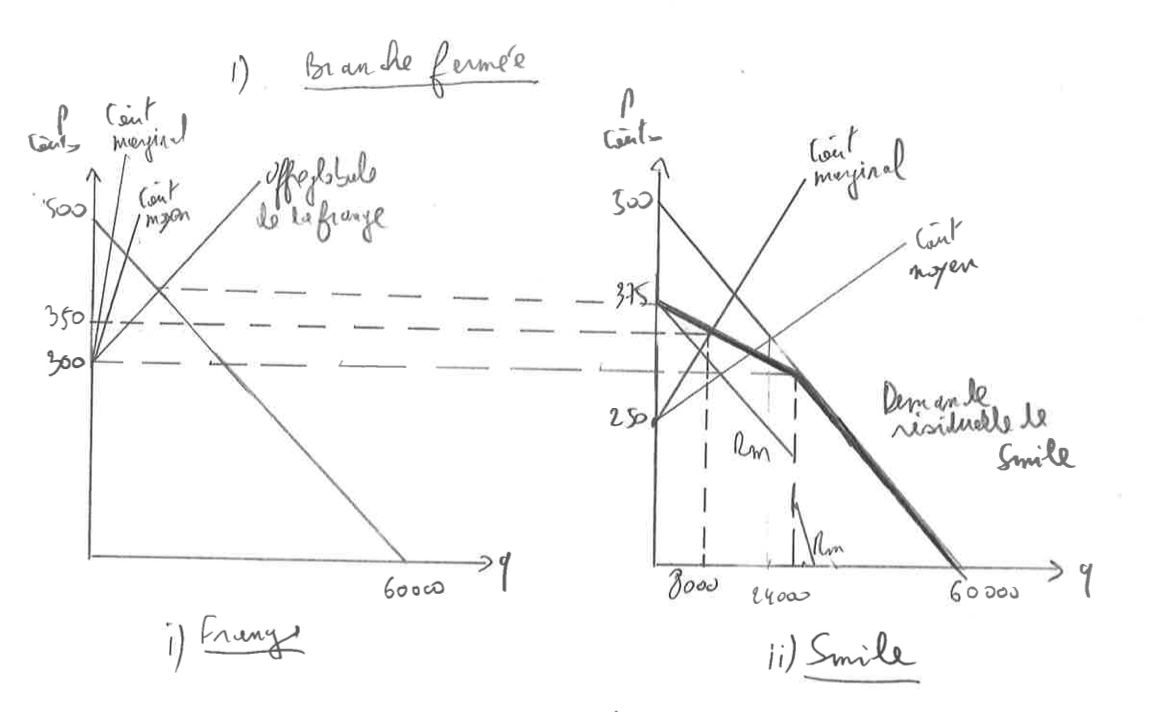
\includegraphics[width=4in]{figq3.png}
   \end{center}
   \end{frame}
   
   \begin{frame}[allowframebreaks]{\insertsection}
   \framesubtitle{Question 10}
   \begin{center}
   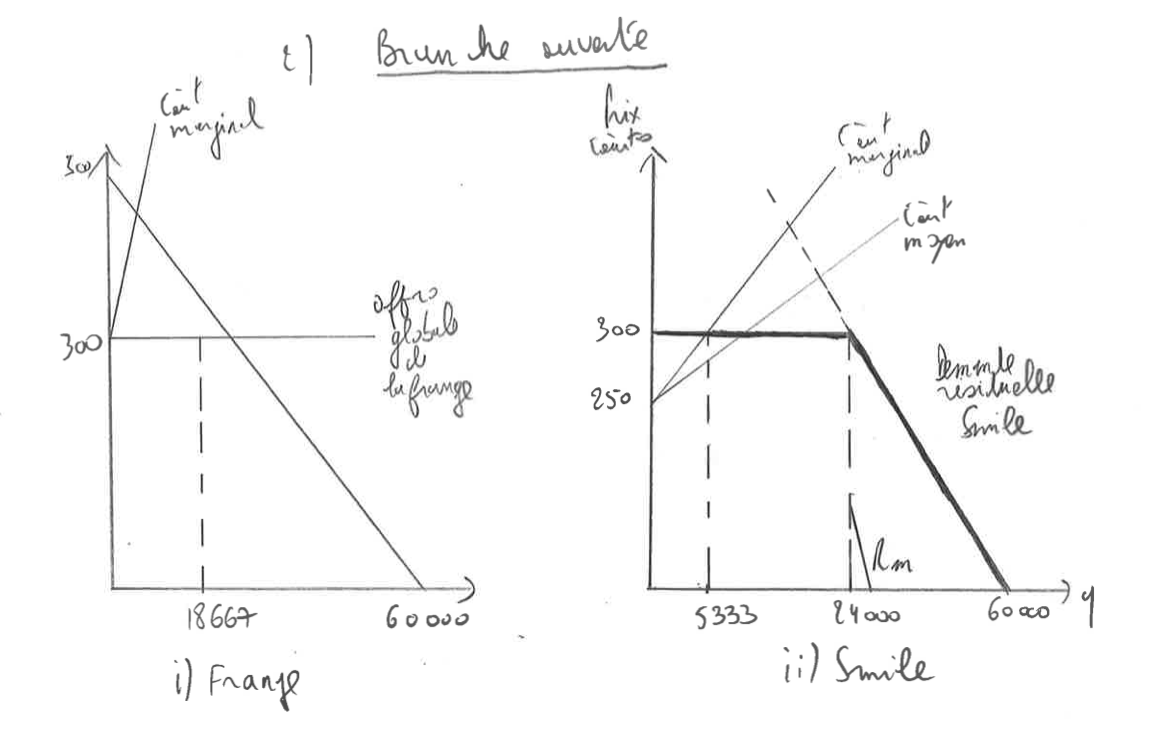
\includegraphics[width=4in]{figq10.png}
   \end{center}
   \end{frame}
   
\begin{frame}[allowframebreaks]{Références}
\bibliographystyle{jpe}
\bibliography{../../../Biblio}
\end{frame}

\end{document}
